\documentclass{beamer}


% \usepackage{CJKnumb}\usepackage{beamerthemesplit}

\mode<article>
{
  \usepackage{beamerbasearticle}
  \usepackage{fullpage}
  \usepackage{hyperref}
}

\usepackage{algorithm}
\usepackage{algorithmic}

%\usepackage{beamerthemesplit} 
%\usepackage{beamerthemeshadow}  
%\usepackage[width=2cm,dark,tab]{beamerthemesidebar}


% Setup appearance:

%\usetheme{Darmstadt}
\usefonttheme[onlylarge]{structurebold}
\setbeamerfont*{frametitle}{size=\normalsize,series=\bfseries}
\setbeamertemplate{navigation symbols}{}

\renewcommand\arraystretch{1.5}

% Standard packages

\usepackage[english]{babel}
%\usepackage[latin1]{inputenc}

\usepackage{epsf}
\usepackage{amsmath,amssymb}
\usepackage{graphicx}
\usepackage{tabularx}

% \usepackage[usenames,dvipsnames]{color}
\definecolor{shadow}{gray}{0.8}
\newcommand{\redc}[1]{{\color{red} #1}}
\newcommand{\bluec}[1]{{\color{blue} #1}}
\newcommand{\shadowc}[1]{{\color{shadow} #1}}
\definecolor{myyellow}{HTML}{FFB700}
\newcommand{\yellowc}[1]{{\color{myyellow} #1}}
\newcommand{\greenc}[1]{{\color{green} #1}}
\newcommand{\vect}[1]{\textbf{\textit{#1}}}
\newcommand{\dd}[1]{\textrm{d}}

\newcommand{\AT}{{\textrm{{AT}}}}
\newcommand{\EX}{{\textrm{EX}}}
\newcommand{\CG}{{\textrm{CG}}}
\newcommand{\HY}{{\Delta}}
\newcommand{\rdf}{{\textrm{rdf}}}

\usepackage{amsfonts}
\newcommand{\tickYes}{\checkmark}
\usepackage{pifont}
\newcommand{\tickNo}{\hspace{1pt}\ding{55}}

% \usetheme{Boadilla}
% \usetheme{Copenhagen}
% \usetheme{Madrid}
\usetheme{Singapore}


\begin{document}
\title[]{
Adaptive Resolution Simulation (AdResS): A smooth 
thermodynamic and structural transition from atomistic to coarse-grained 
resolution and vice versa in a grand canonical fashion
}
%
\author{Han Wang}
\institute[FUB] {
  Institute for Mathematics, Freie Universit\"at Berlin, Germany\\
  % Institut f\"ur Mathematik, Freie Universit\"at Berlin, Germany\\
\vskip 0.4cm
Joint with: Carsten Hartmann, Christof Sch\"utte, Luigi Delle Site (FUB) }
\date[2012]{29 August 2012, Lorentz Center (Leiden Univ.)}
\frame{\titlepage}


\begin{frame}{AdResS: the motivation}
  \redc{AdResS} = \redc{Ad}aptive \redc{Res}olution \redc{S}imulation
  \begin{itemize}
  \item Bridging models on different scales.
  \item Capturing both local processes and global behaviors.
  \end{itemize}
  \begin{figure}
    \centering 
    \includegraphics[width=0.4\textwidth]{fig/zoom2.eps}
    % 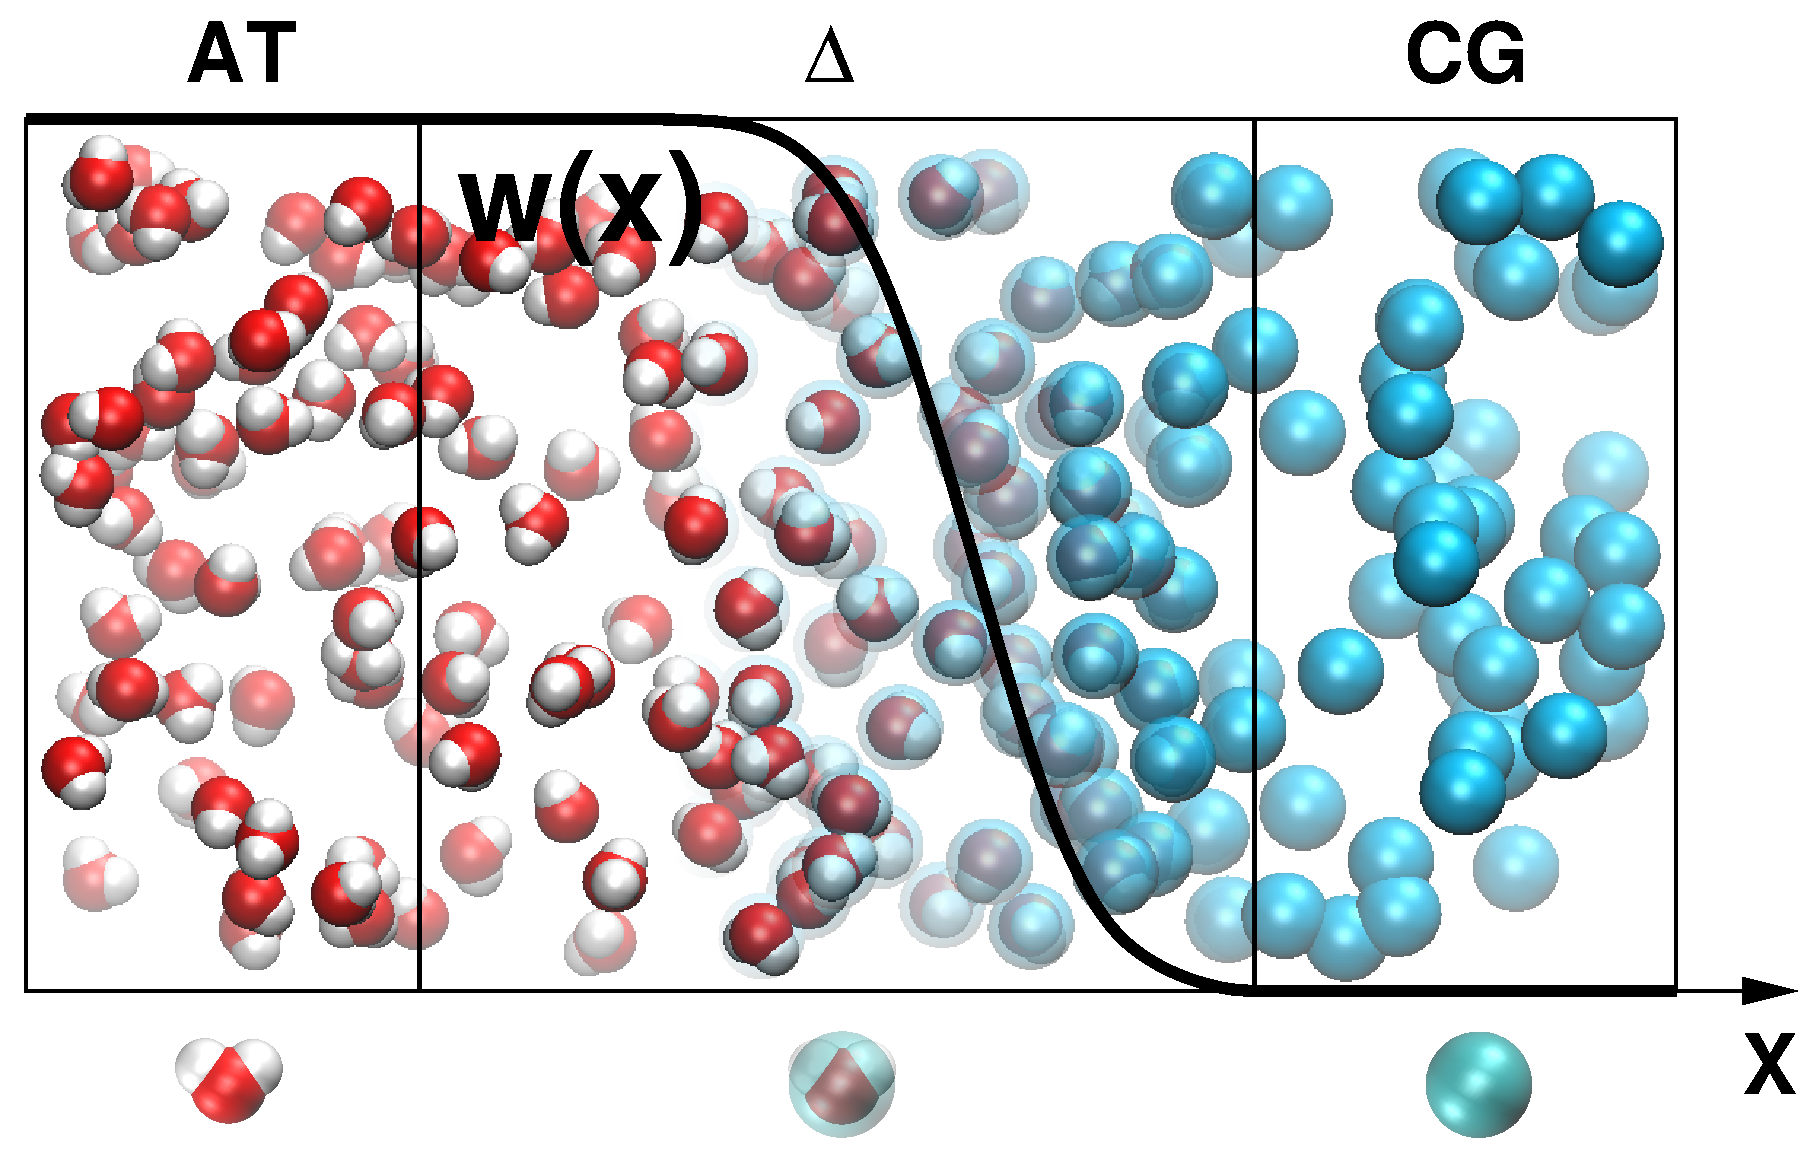
\includegraphics[width=0.8\textwidth]{fig/adapt-wat.eps}
  \end{figure}
\end{frame}

\begin{frame}{Essential principles}
  \vfill
  \vfill
  \begin{itemize}
  \item<1-> \redc{Increase resolution} of molecules in
    a sub-region (keeping the rest at lower resolution).
  \vfill
  \item<2-> \redc{Free exchange} of molecules between resolutions.
  \vfill
  \item<3-> \redc{Thermodynamics equilibrium} is guaranteed.
  \end{itemize}
  \vfill
  \vfill
\end{frame}

\begin{frame}{AdResS, Basic concepts}{Defining the hybrid resolution}
  \begin{figure}
    \centering 
    \includegraphics[width=0.8\textwidth]{fig/system/system-oldw.eps}
    % 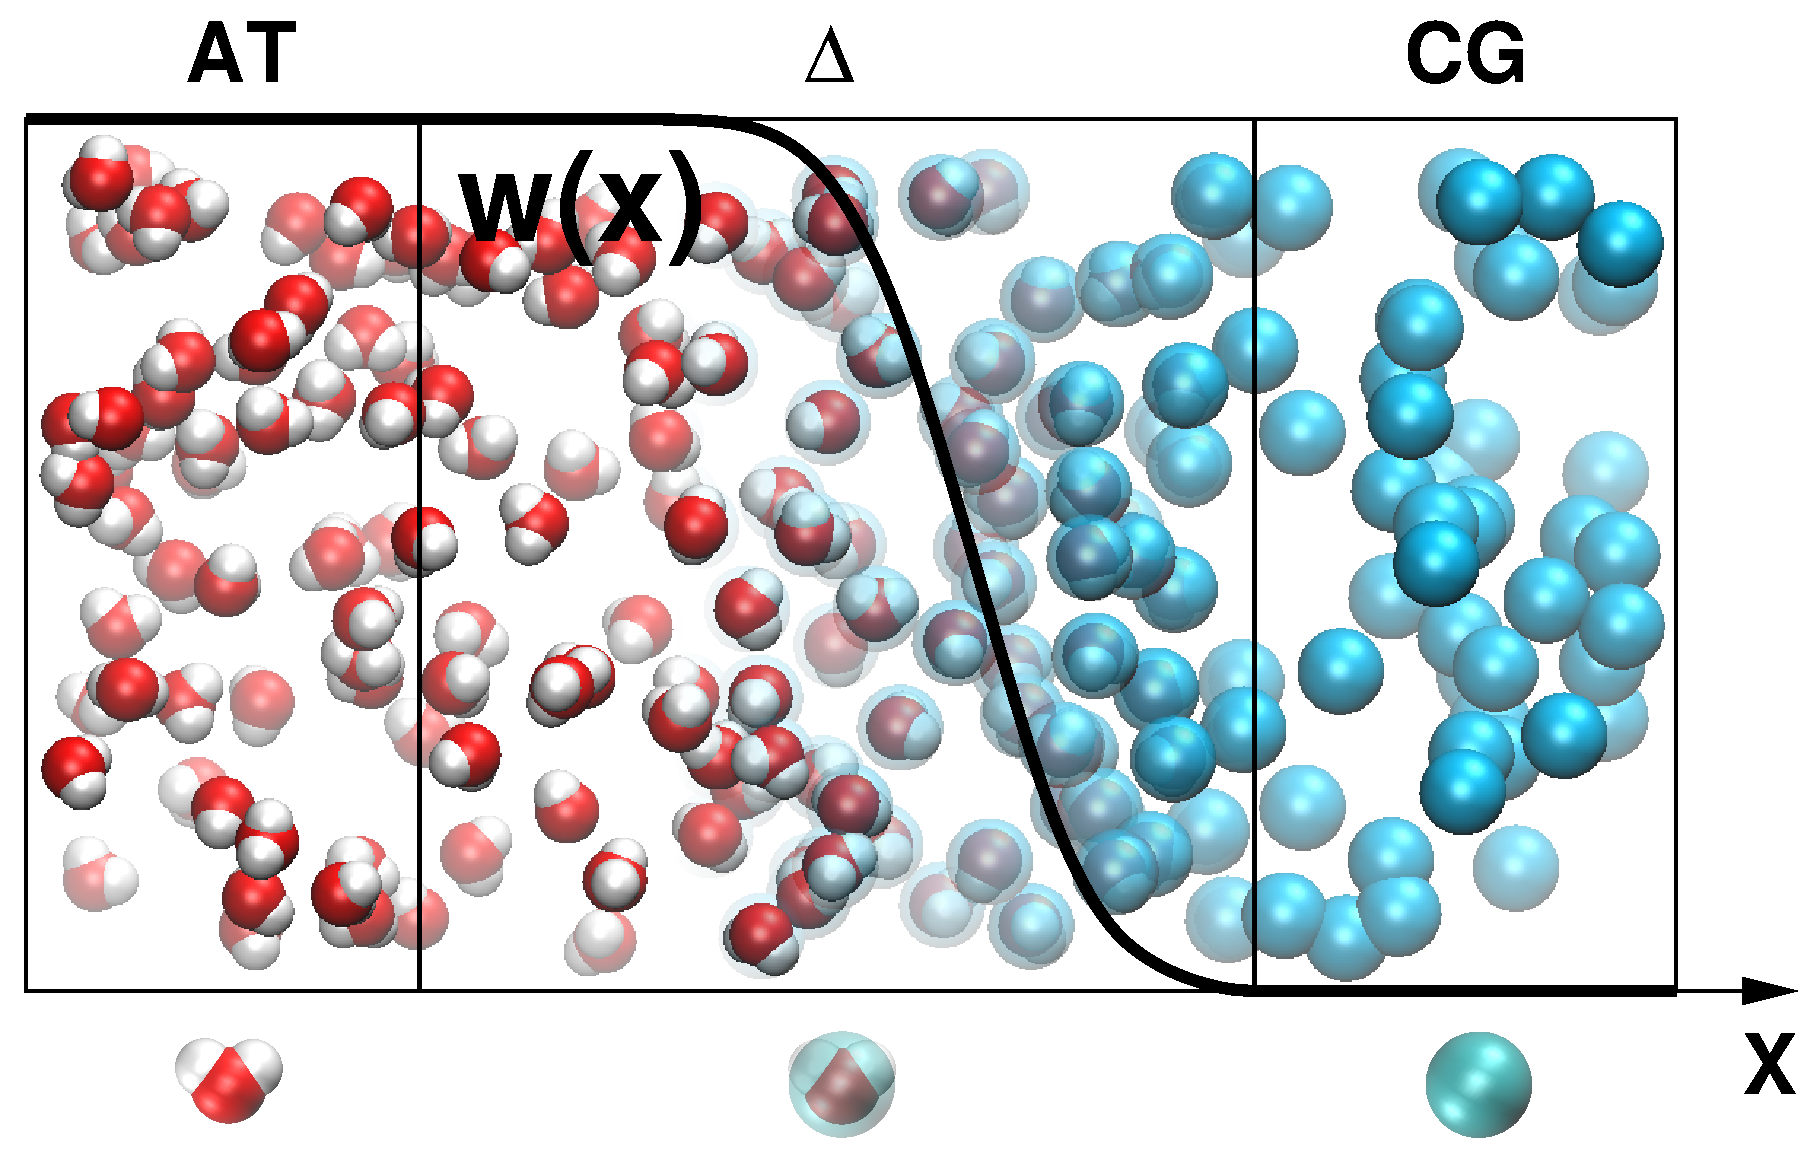
\includegraphics[width=0.8\textwidth]{fig/adapt-wat.eps}
  \end{figure}
  \begin{equation*}
    {\vect F}_{\alpha \beta}=w(x_\alpha)w(x_\beta){\vect F}_{\alpha\beta}^{\AT}+[1-w(x_\alpha)w(x_\beta)]{\vect F}^{\CG}_{\alpha\beta}
  \footnote{M. Praprotnik, L. Delle Site, K. Kremer, JCP \textbf{123}, 224106 (2005)}
  \end{equation*}
\end{frame} 

\begin{frame}{AdResS, Force interpolation}
  \begin{figure}
    \centering 
    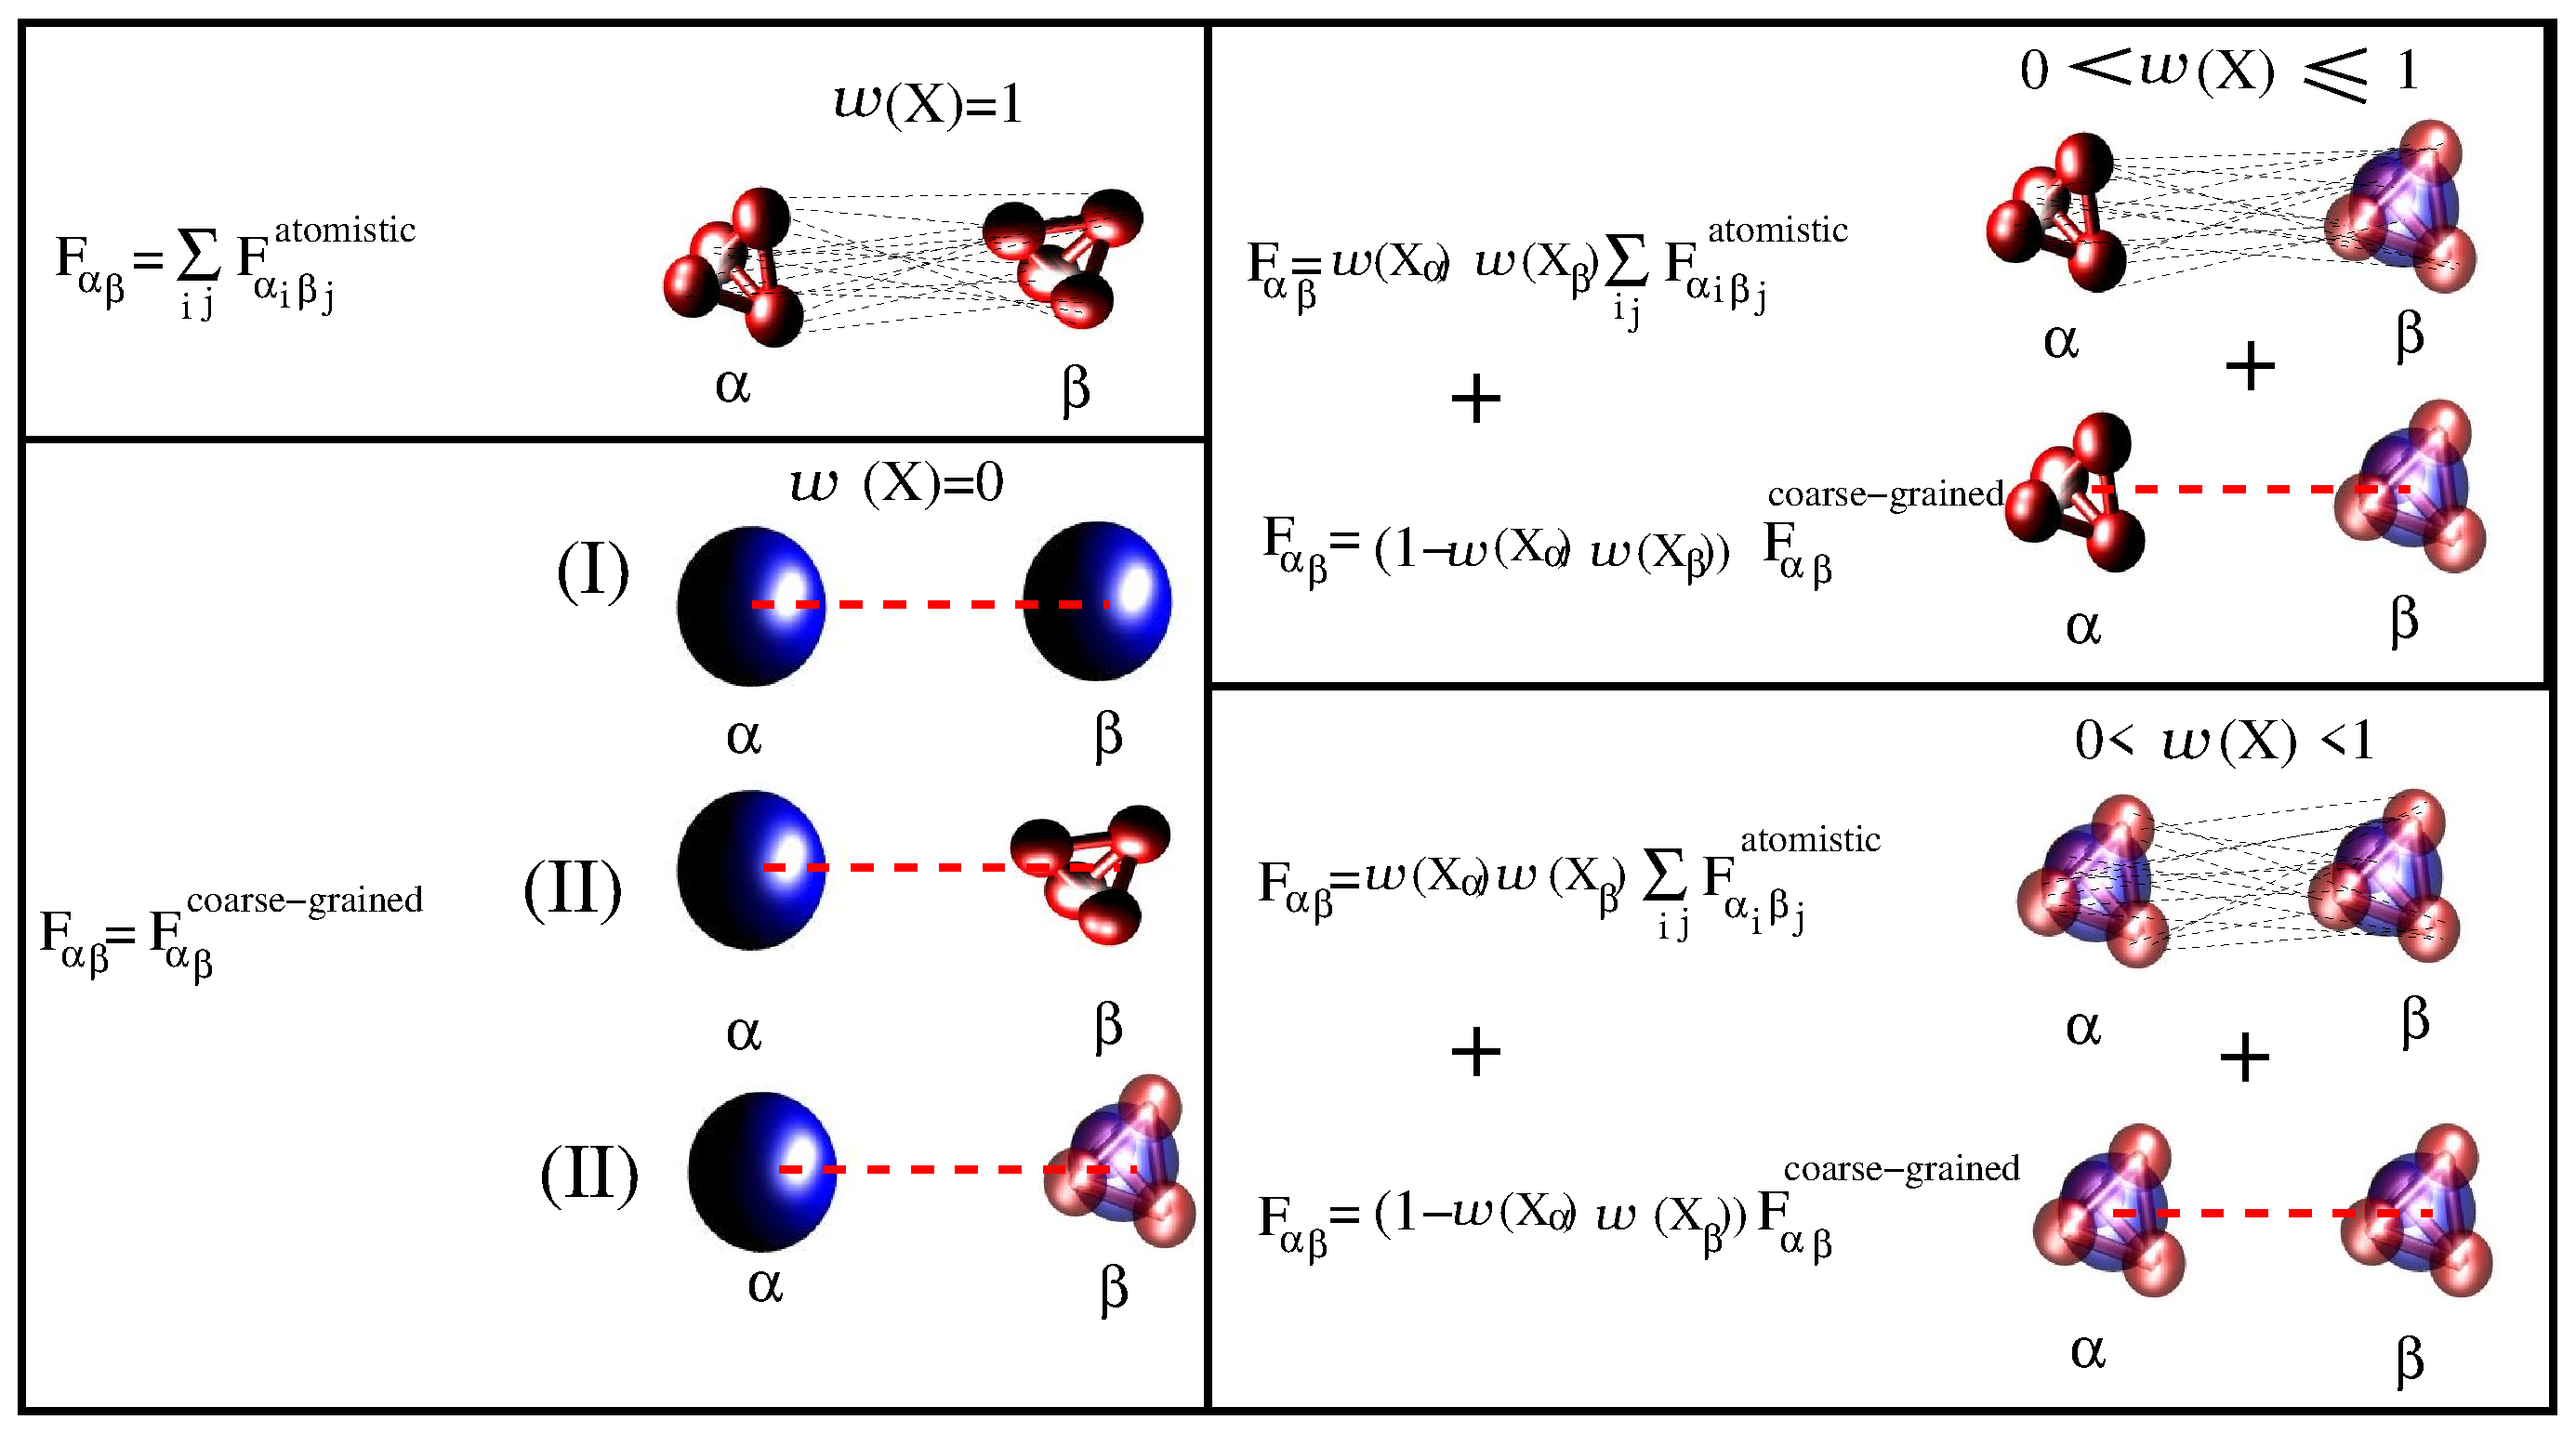
\includegraphics[width=0.99\textwidth]{fig/force.eps}
  \end{figure}
  \begin{equation*}
    {\vect F}_{\alpha \beta}=w(x_\alpha)w(x_\beta){\vect F}_{\alpha\beta}^{\AT}+[1-w(x_\alpha)w(x_\beta)]{\vect F}^{\CG}_{\alpha\beta}
  \end{equation*}
\end{frame} 


\begin{frame}{The thermodynamic equilibrium}
  The thermodynamic equilibrium:
  \begin{itemize}
  \item $\rho_{\CG} = \rho_{\AT}$
  \item $P_{\CG} = P_{\AT}$
  \item $T_{\CG} = T_{\AT}$
  \item $\mu_{\CG} = \mu_{\AT}$
  \item ...
  \end{itemize}
  \vskip .5cm
  \redc{Representability problem} of coarse graining, see e.g.
  Ref.\footnote{M.E. Johnson, T. Head-Gordon, A.A. Louis, JCP \textbf{126}, 144509 (2007).}\\
  \begin{itemize}
  \item $g_{\CG}(r) = g_{\AT}(r)$
    {($\Longrightarrow \kappa_{\CG} = \kappa_{\AT},\
      P_{\CG} \neq P_{\AT}$)}
  \item \redc{or} $P_{\CG} = P_{\AT}$ \bluec{\ \ \ losing the accuracy of $g(r)$ \& $\kappa$\footnote{H. Wang, C. Junghans, K. Kremer, EPJ-E \textbf{28}, 221 (2009)}}
  \end{itemize}
\end{frame}



\begin{frame}{Coupling the two resolutions by matching the pressure}
  \begin{itemize}
  \item 
    Pressure corrected coarse-grained model,\\
  \item 
    \bluec{wrong density profile in hybrid region...\footnote{
      S. Poblete, M. Praprotnik, K. Kremer, L. Delle Site, JCP \textbf{132}, 114101 (2010). Figure
      with courtesy of L. Delle Site
    }}
    \begin{minipage}[t]{0.78\linewidth}
      \begin{figure}
        \includegraphics[width=1.\textwidth]{fig/pcorr-rho.eps}\hfill
      \end{figure}
    \end{minipage}\\
  \end{itemize}
\end{frame}



\begin{frame}{Coupling the two resolutions by matching RDF}
  \begin{itemize}
    \vfill
  \item <1-> Use the structurally correct coarse-grained model (fit $g(r)$): 
    \redc{$g_{\AT}(r) =  g_{\CG}(r)$}; \redc{$\kappa_{\AT} =  \kappa_{\CG}$}
    \vfill
  \item 
    \vfill
    \bluec{$P_{\AT}\neq P_{\CG} \Longrightarrow \rho_{\AT}\neq \rho_{\CG}$}; 
    \begin{figure}
      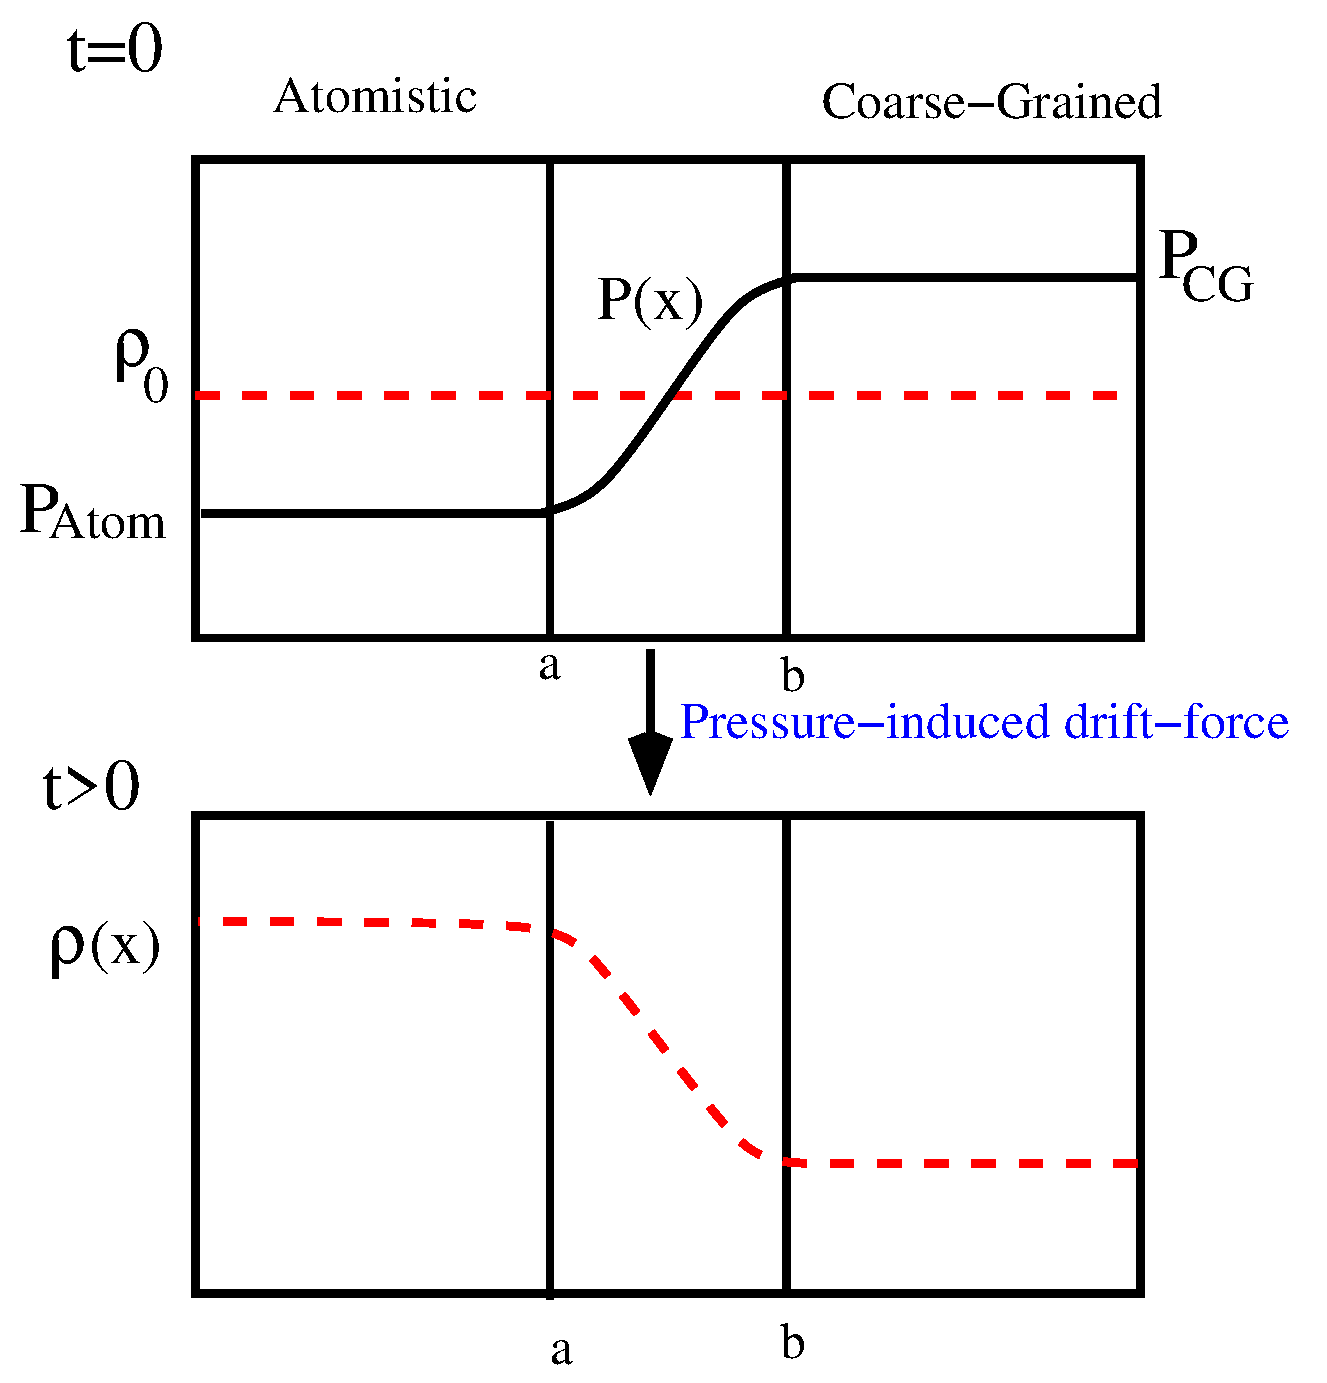
\includegraphics[width=.5\textwidth]{fig/pressure.eps}
    \end{figure}    
  % \item <2-> The ``thermodynamic force'':
  %   \begin{align*}
  %     &-\left[P_{AT}+ \frac{\rho_{0}}{M_\alpha}\int_{\Delta} \redc{{\vect F}^\text{th}(x)}\,\text{d}x\right] V = -P_{CG}V; \\
  %     &{\vect F}_{\alpha}=\sum_{\beta}{\vect F}_{\alpha\beta}+{\vect F}^{\textrm{th}}(x_{\alpha}).
  %   \end{align*}
  %   \vfill
  % \item <3-> Is AdResS a \redc{grand canonical} simulation:
  %   \begin{align*}
  %     p(\vect x, N) = \frac{1}{\mathcal Z}
  %     e^{\beta\mu_{AT} N - \beta \mathcal H^{AT}(\vect x)} \quad (?)
  %   \end{align*}
  %   \vfill
  \end{itemize}
\end{frame}

\begin{frame}{Solution: the thermodynamic force}
  \begin{itemize}
  \item <1-> The ``thermodynamic force''\footnote{S. Fritsch, et.al. PRL \textbf{108}, 170602 (2012)}:
    \begin{align*}
      &-\left[P_{AT}+ \frac{\rho_{0}}{M_\alpha}\int_{\Delta} \redc{{\vect F}^\text{th}(x)}\,\text{d}x\right] V = -P_{CG}V; \\
    \end{align*}
  \item Iterative procedure (TFI):
    \begin{equation*}
      {\vect F}_{k+1}^{\textrm{th}}(x)={\vect F}_{k}^{\textrm{th}}(x)-\frac{M_{\alpha}}{[\rho_{0}]^{2}\kappa}\nabla\rho_{k}(x)
      \label{iter}
    \end{equation*}
  \item Scheme:
    \begin{align*}
      &{\vect F}_{\alpha}=\sum_{\beta}{\vect F}_{\alpha\beta}+{\vect F}^{\textrm{th}}(x_{\alpha}).
    \end{align*}
  \end{itemize}
\end{frame}


\begin{frame}{Thermodynamic force: numerical results
    \footnote{S. Fritsch, et.al. PRL \textbf{108}, 170602 (2012), Figs.
    with courtesy of L. Delle Site}}
  \begin{figure}
    \includegraphics[width=.5\textwidth]{fig/spce_all.eps}\hfill
    \includegraphics[width=.5\textwidth]{fig/part_dist.eps}\hfill
  \end{figure}  
\end{frame}


\begin{frame}{Consequence of the thermodynamic force}
  \begin{itemize}
    \vfill
  \item<1-> Consequence:\\
    \redc{
      \vskip -.8cm
      \begin{align*}
        \rho_{\AT} &=  \rho_{\CG}\\
        \kappa_{\AT} &= \kappa_{\CG}
      \end{align*}
    }
    \bluec{
      \vskip -1.6cm
      \begin{align*}
        P_{\AT}& \neq P_{\CG}\\
        \mu_{\AT}& \neq  \mu_{\CG}
      \end{align*}
    }
    \vskip -5.0cm
    % \redc{$\rho_{\AT}(r) =  \rho_{\CG}(r)$};\\
    % \redc{$\kappa_{\AT} =  \kappa_{\CG}$}\\
    % \bluec{$P_{\AT}(r) \neq P_{\CG}(r)$};\\
    % \bluec{$\mu_{\AT} \neq  \mu_{\CG}$}
    % \vfill
  \item<2-> The {thermodynamic work $w_0$} generated/adsorbed by ${\vect F}^\text{th} (x)$ removes the
    differences and assures the equilibrium.\footnote{H. Wang, C. Hartmann, C. Sch\"utte, L. Delle Site, in preparation (2012)}
    \redc{
    \begin{align*}
      w_0 &= \mu_{\CG} - \mu_{\AT}\\
      \rho_0 w_0 &= P_{\CG} - P_{\AT}
    \end{align*}}
  \end{itemize}
    \vfill
\end{frame}


\begin{frame}{$\HY$ region: smoothly bridging two resolutions / embeded as if
  in a full atomistic environment}
  \begin{align*}
    \rho_{\AT} = &\,\rho_{\HY} = \rho_{\CG} \\
    \redc{g_{AT}(r) =} &\redc{\,g_{\HY}(r) = g_{\CG}(r) }
  \end{align*}
  \begin{figure}
    \centering 
    \includegraphics[width=0.7\textwidth]{fig/system/system-oldw.eps}
    % 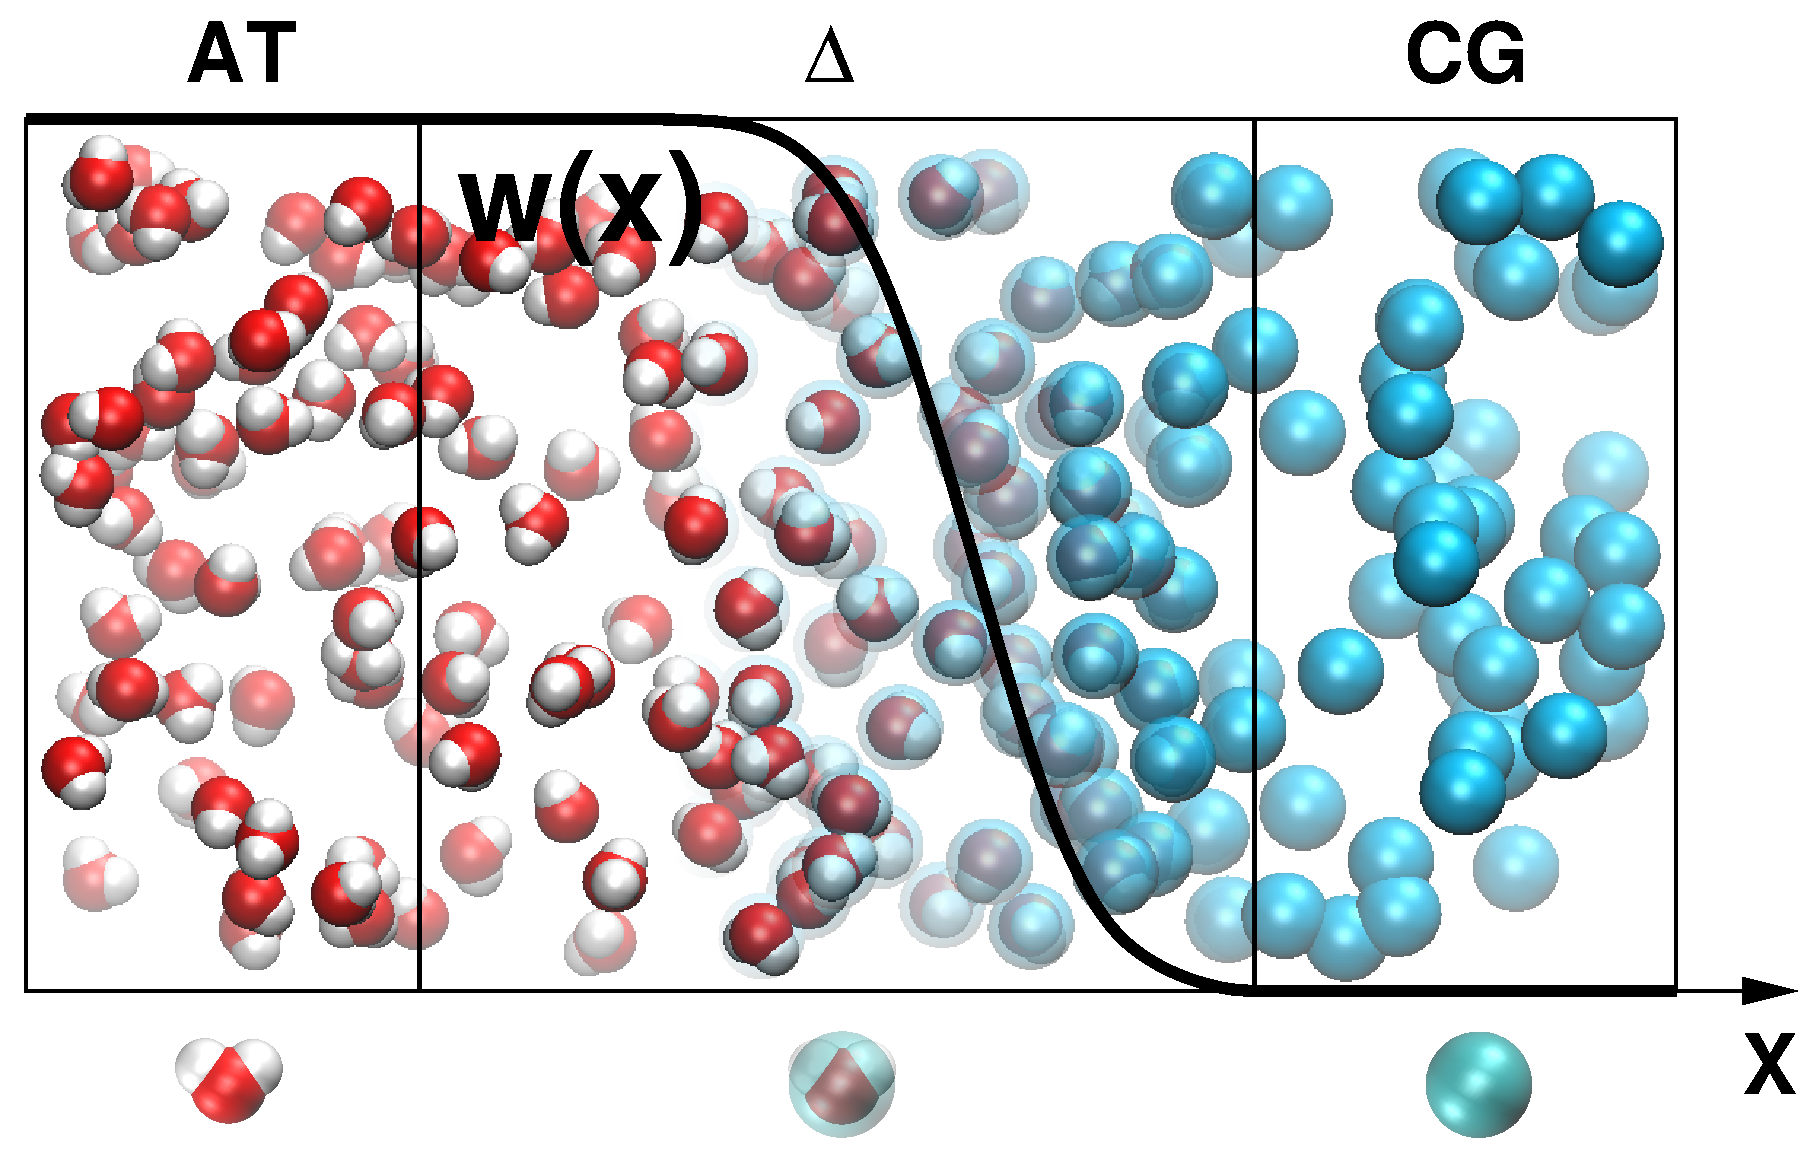
\includegraphics[width=0.8\textwidth]{fig/adapt-wat.eps}
  \end{figure}
\end{frame}


\begin{frame}{The COM RDF correction in the $\HY$ region}
  \vfill
  Basic requirements for the correction:
  \begin{enumerate}
  \item It should \redc{only act} in $\HY$ region.
  \item It should \redc{not perturb} the overall equilibrium
  \item \redc{Low} extra computational cost.
  \end{enumerate}
  \vfill
  Pairwise correction force in $\HY$, scheme:\footnote{H. Wang, C. Sch\"uette, L. Delle Site, JCTC \textbf{8}, 2878 (2012)}
  \begin{align*}
    \vect F_{\alpha\beta}
    &=
    w_\alpha w_\beta \vect F_{\alpha\beta}^{\AT} +
    (1 - w_\alpha w_\beta) \vect F_{\alpha\beta}^{\CG} +
    \redc{w_\alpha w_\beta (1 - w_\alpha w_\beta) \vect F_{\alpha\beta}^{\rdf}}
  \end{align*}
  \vskip -.6cm
  \begin{align*}
    {\vect F}_{\alpha}
    &=
    \sum_{\beta}{\vect F}_{\alpha\beta}+{\vect F}^{\textrm{th}}(x_{\alpha}).    
  \end{align*}
  \vfill
\end{frame}


\begin{frame}{``Extension'' of the hybrid region}
  \begin{figure}
    \centering 
    \includegraphics[width=0.8\textwidth]{fig/system/system-neww.eps}
  \end{figure}
\end{frame} 

\begin{frame}{IBI algorithm to calculate $\vect F^\rdf$}
  step 0:
  \begin{align*}
    U^{\textrm{rdf}}_0(r)
    = -k_BT\ln g_{{\AT}}(r)
  \end{align*}
  step 1:
  \begin{align*}\label{eqn:ibi}
    U^{\textrm{rdf}}_{k+1}(r) = U^{\textrm{rdf}}_k(r) +
    k_B T\ln\bigg[
    \frac{g_k(r)}{g_{{\AT}}(r)}
    \bigg]
  \end{align*}
  step 2:
  \begin{align*}
    \vect F^{\textrm{rdf}}_{\alpha\beta} = \vect F_{k+1}^{\textrm{rdf}}(\vect r_{\alpha\beta})
    = -\nabla_{\vect r}\,U_{k+1}(r_{\alpha\beta}).
  \end{align*}
\end{frame}

\begin{frame}{IBI-TFI correction loop}
  \begin{figure}
    \centering 
    \includegraphics[width=0.8\textwidth]{fig/algorithm.pdf}
  \end{figure}
\end{frame}

\begin{frame}{Resulting RDF: SPC/E water}
  \begin{figure}
    \centering 
    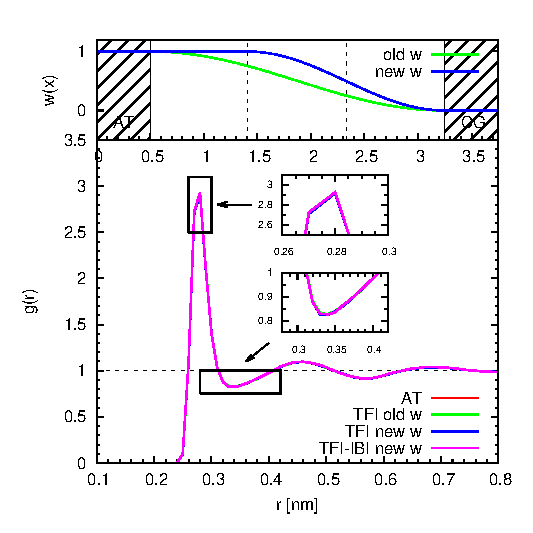
\includegraphics[width=0.7\textwidth]{fig/rdf-ex-cg.eps}
  \end{figure}  
\end{frame}

\begin{frame}{Resulting RDF}
  \begin{figure}
    \centering 
    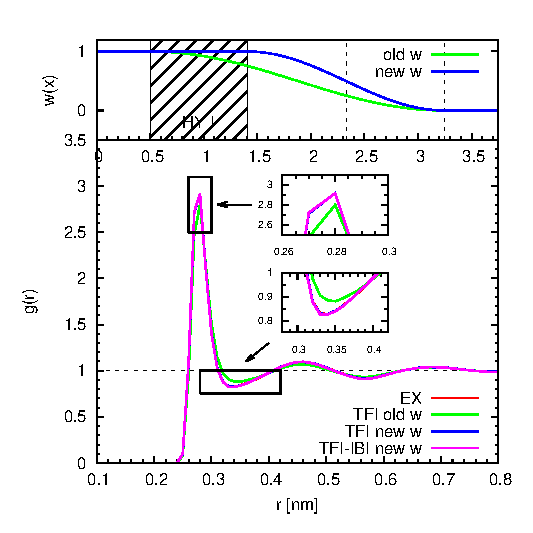
\includegraphics[width=0.7\textwidth]{fig/rdf-425-516.eps}
  \end{figure}  
\end{frame}

\begin{frame}{Resulting RDF}
  \begin{figure}
    \centering 
    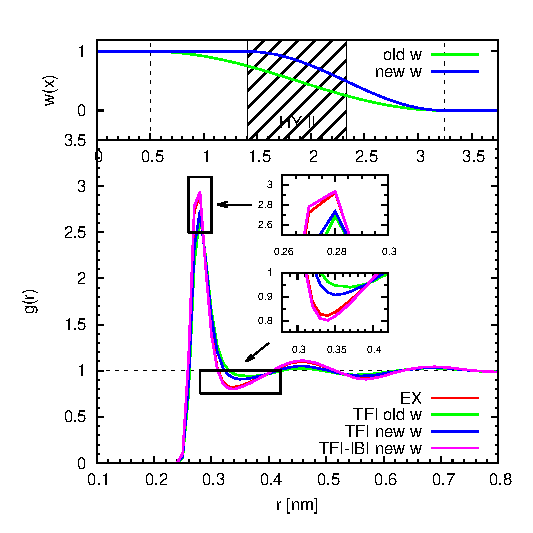
\includegraphics[width=0.7\textwidth]{fig/rdf-516-608.eps}
  \end{figure}  
\end{frame}

\begin{frame}{Resulting RDF}
  \begin{figure}
    \centering 
    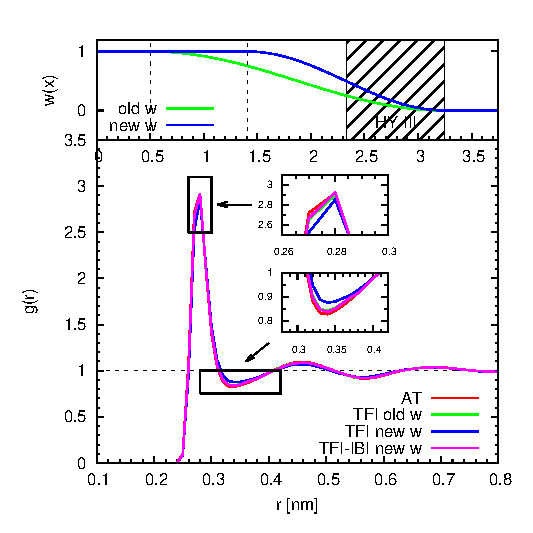
\includegraphics[width=0.7\textwidth]{fig/rdf-608-700.eps}
  \end{figure}  
\end{frame}


\begin{frame}{The RDF correction force}
  \begin{figure}
    \centering 
    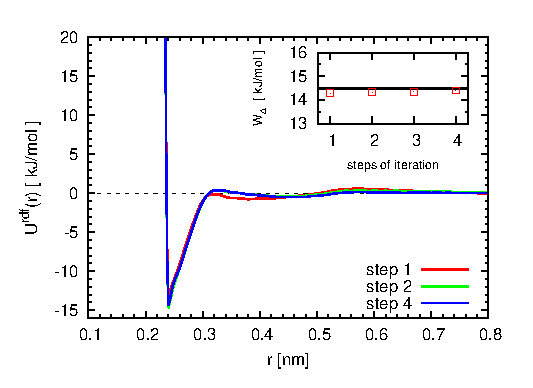
\includegraphics[width=0.8\textwidth]{fig/force-rdf.eps}
  \end{figure}    
\end{frame}

\begin{frame}{The density}
  \begin{figure}
    \centering 
    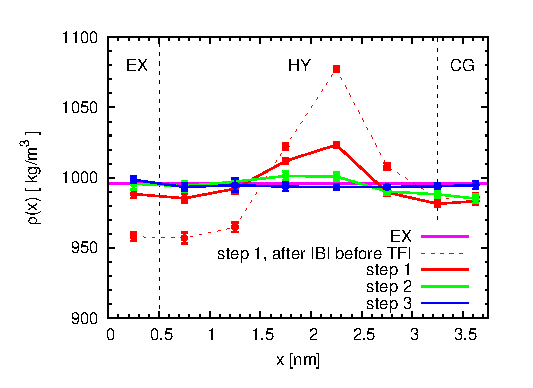
\includegraphics[width=0.8\textwidth]{fig/rho.eps}
  \end{figure}    
\end{frame}

\begin{frame}{The number fluctuation}
  \begin{figure}
    \centering 
    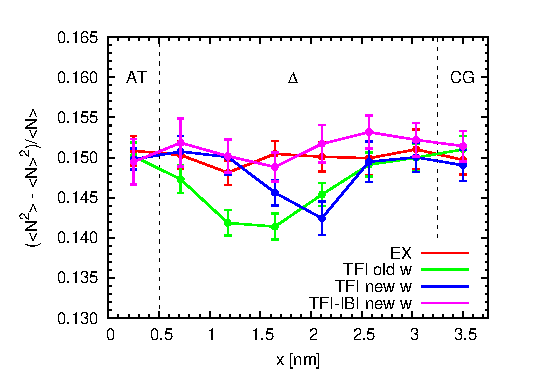
\includegraphics[width=0.8\textwidth]{fig/count.eps}
  \end{figure}    
\end{frame}



\begin{frame}{AdResS as an effective grand canonical sampling}
  \begin{itemize}
  \item<1->     \AT: $\vect x_1; N_1$,
    $\HY$: $\vect x_2; N_2$,
    \CG: $\vect x_3; N_3$.\\
  \item <2-> 
    The target is:
    \begin{align*}
      p(\vect x_1, N_1) = \frac{1}{\mathcal Z_1}
      e^{\beta\mu_{AT} N_1 - \beta \mathcal H^{AT}(\vect x_1)} 
    \end{align*}
  \item <3-> Decomposition:
    \begin{align*}
      p(\vect x_1, N_1) = p(\vect x_1 | N_1) \,{p (N_1)}
    \end{align*}
    we study:
    \redc{
    \begin{align*}
      p(\vect x_1 | N_1) &= \frac{1}{Z_{N_1}} e^{-\beta \mathcal H^{AT}(\vect x_1)} \\
      p(N_1) &= \frac{1}{\mathcal Z_1}e^{\beta\mu_{AT} N_1}Z_{N_1}
    \end{align*}}
  \end{itemize}  
\end{frame}

\begin{frame} {The full atomistic reference system}
  \begin{figure}
    \centering 
    \includegraphics[width=0.5\textwidth]{fig/system/system-full-atom-1.eps}\\
    \vfill
    \includegraphics[width=0.5\textwidth]{fig/system/system-neww.eps}
  \end{figure}      
\end{frame}

\begin{frame}{$p(\vect x_1 | N_1)= \frac{1}{Z_{N_1}} e^{-\beta \mathcal H^{AT}(\vect x_1)} $}
  \vfill
  Correct embedment of AT in the AdResS system:
  \begin{itemize}
  \item Interacting with $\HY$ in an \redc{atomistic way}.
  \item \redc{Correct distribution} in $\HY$.
  \end{itemize}
  \vfill
  Math translation:
    \begin{align*}
      &p(\vect x_1 | N_1) = \sum_{N_2}\int
      p(\vect x_1 | N_1; \vect x_2, N_2) \,
      p(\vect x_2, N_2 | N_1)
      \,\dd d\vect x_2\\
      &p(\vect x_1 | N_1; \vect x_2, N_2)
      = \, \frac 1{Z(\vect x_2, N_2)}
      e^{-\beta\redc{\mathcal H^{AT}(\vect x_1; \vect x_2, N_2)}}\\
      &p(\vect x_2, N_2 | N_1)
      \longrightarrow
      \redc{\rho_\HY = \rho_\AT,\quad
      g_\HY(r) = g_\AT(r)}
    \end{align*}
  \vfill
\end{frame}


\begin{frame}{$p(N_1)$}
  \begin{itemize}
    \vfill
  \item <1-> the probability of $N_1$: 
    \begin{align*}
      p(\vect x_1, N_1) = p(\vect x_1 | N_1) \, \redc{p (N_1)}
    \end{align*}
    \vfill
  \item <2-> Assumptions:
    \vfill
    \begin{itemize}
    \item thermodynamics limit: $N_2\ \bluec{\ll}\ N_1 \ll N_3$
      \vfill
    \item additive Hamiltonian of AT and CG regions:\\
        \vskip -.5cm
      \begin{equation*}
        \mathcal H(\vect x_1, N_1; \vect x_3, N_3) =
        \mathcal H^{\AT}(\vect x_1, N_1) + \mathcal H^{\CG}(\vect x_3, N_3); \qquad N_1 + N_3 = N
      \end{equation*}
    \end{itemize}
    \vfill
  \item <3-> Accuracy\footnote{H. Wang, C. Hartmann, C. Sch\"utte, L. Delle Site, in preparation (2012)}:
    \vfill
    \begin{itemize}
    \item \redc{Convergent}
    \vfill
    \item First order: \redc{$\mu_{\AT} = \mu_{\CG} - w_0$}
      $\leftarrow$ thermodynamics force.
    \vfill
  \item Second order: \redc{$\kappa_{\AT} = \kappa_{\CG}$}
    $\leftarrow g_{\AT}(r) = g_{\CG}(r)$.
    \end{itemize}
    \vfill
  \end{itemize}
\end{frame}


\begin{frame}{Further numerical verification}
  We want to check the marginal distributions of $p(\vect x_1, N_1)$
  \begin{itemize}
    \vfill
  \item <1-> $p(N_1)$
    \vfill
    \begin{enumerate}
    \item  $\langle N_1\rangle$.
      \vfill
    \item  $\langle [\delta N_1]^2\rangle$.
    \end{enumerate}
    \vfill
  \item <2-> $p(\vect x_1)$
    \begin{itemize}
    \vfill
    \item  $\rho(r)$
      \vfill
    \item $g(r)$ (center-of-mass RDF)
      \vfill
    \item \redc{$g_{HH}(r)$, $g_{OH}(r)$}
      \vfill
    \item \redc{$g^{(3)} (\vect r_1, \vect r_2, \vect r_3)$}
    \end{itemize}
    \vfill
  \end{itemize}
\end{frame}



\begin{frame}{$g_{HH}(r)$ \& $g_{OH}(r)$}
  \begin{figure}
    \centering 
    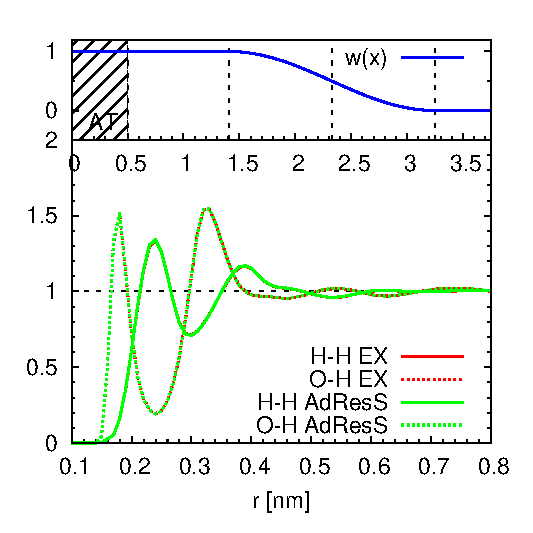
\includegraphics[width=0.7\textwidth]{fig/rdf-hhoh-375-425.eps}
  \end{figure}    
\end{frame}

\begin{frame}{$g_{HH}(r)$ \& $g_{OH}(r)$}
  \begin{figure}
    \centering 
    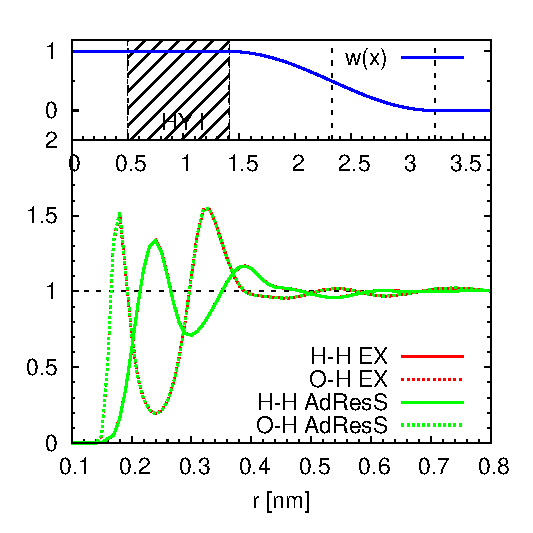
\includegraphics[width=0.7\textwidth]{fig/rdf-hhoh-425-516.eps}
  \end{figure}    
\end{frame}

\begin{frame}{$g_{HH}(r)$ \& $g_{OH}(r)$}
  \begin{figure}
    \centering 
    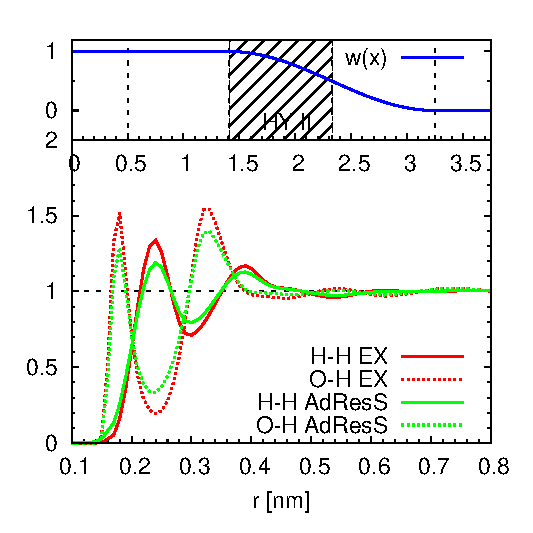
\includegraphics[width=0.7\textwidth]{fig/rdf-hhoh-516-608.eps}
  \end{figure}    
\end{frame}

\begin{frame}{$g_{HH}(r)$ \& $g_{OH}(r)$}
  \begin{figure}
    \centering 
    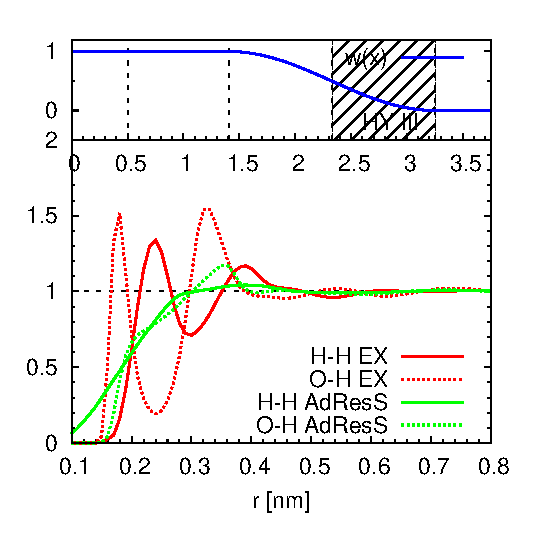
\includegraphics[width=0.7\textwidth]{fig/rdf-hhoh-608-700.eps}
  \end{figure}    
\end{frame}


\begin{frame}{$g^3(\vect r_1, \vect r_2, \vect r_3)$, the definition}
  \begin{figure}
    \centering
    \includegraphics[width=0.5\textwidth]{fig/3mol.eps}
  \end{figure}
  The 3-body RDF is defined by
  \begin{align*}
    g^{(3)}(\vect r_1, \vect r_2, \vect r_3) =
    \frac{1}{\rho^3}N(N-1)(N-2) \,p^{(3)}(\vect r_1, \vect r_2, \vect r_3) 
  \end{align*}
\end{frame}

\begin{frame}{Reproducing the $g^3(\vect r_1, \vect r_2, \vect r_3)$}
  \begin{figure}
    \centering 
    \includegraphics[width=0.9\textwidth]{fig/fig-rdf3-more-eps-converted-to-1.pdf}
    % \includegraphics[width=0.9\textwidth]{fig/fig-rdf3-more.eps}
  \end{figure}    
\end{frame}


\begin{frame}{AdResS: bridging the quantum and classical resolutions}
  \begin{itemize}
  \item   Liquid tetrahedral molecules.\footnote{
      A.B. Poma, L. Delle Site, PRL \textbf{104}, 250201 }
    \begin{minipage}[m]{0.58\linewidth}
      \begin{figure}
        \includegraphics[width=0.9\textwidth]{fig/switching.eps}
      \end{figure}
    \end{minipage}
    \begin{minipage}[m]{0.28\linewidth}
      \begin{figure}
        \includegraphics[width=1.6\textwidth]{fig/3plot.pdf}
      \end{figure}
    \end{minipage}\hfill
  \item Applications to liquid para-hydrogen.\footnote{
      A.B. Poma, L. Delle Site, PCCP \textbf{13} 10510 (2011) \&
      R. Potestio, L. Delle Site, JCP \textbf{136}, 054101 (2012).}
  \end{itemize}
\end{frame}









% \begin{frame}{Proof}
%   \begin{itemize}
%   \item <1-> Notation:\\
%     atomistic $\vect x_1; N_1$,
%     hybrid $\vect x_2; N_2$,
%     coarse-grained $\vect x_3; N_3$.\\
%     so the target is:
%     \begin{align*}
%       p(\vect x_1, N_1) = \frac{1}{\mathcal Z_1}
%       e^{\beta\mu_{AT} N_1 - \beta \mathcal H^{AT}(\vect x_1)} 
%     \end{align*}
%   \item <2-> Firstly, fix the number of molecules in atomistic region:
%     \begin{align*}
%       p(\vect x_1, N_1) = p(\vect x_1 | N_1) \,{p (N_1)}
%     \end{align*}
%     we should prove:
%     \begin{align*}
%       p(\vect x_1 | N_1) &= \frac{1}{Z_{N_1}} e^{-\beta \mathcal H^{AT}(\vect x_1)} \\
%       p(N_1) &= \frac{1}{\mathcal Z_1}e^{\beta\mu_{AT} N_1}Z_{N_1}
%     \end{align*}
%   \end{itemize}
% \end{frame}

% \begin{frame}{Proof}
%   \begin{itemize}
%   \item <1-> The atomistic region is a sub system embedded in the
%     hybrid region.
%     \begin{align*}
%       p(\vect x_1 | N_1) = \sum_{N_2}\int
%       p(\vect x_1 | N_1; \vect x_2, N_2) \,
%       p(\vect x_2, N_2 | N_1)
%       \,\d d\vect x_2
%     \end{align*}
%   \item <2-> Fortunately, we have
%     \begin{align*}
%       p(\vect x_1 | N_1; \vect x_2, N_2)
%       \propto &\,
%       e^{-\beta\mathcal H^{AT}(\vect x_1; \vect x_2, N_2)}
%       \quad \redc{\textrm{AT probability!!}}\\
%       \mathcal H^{{AT}}(\vect x_1; \vect x_2, N_2) = &\,
%       \sum_{j=1}^{N_1}\frac12 m_i\vect v_i^2 + 
%       \sum_{i,j=1}^{N_1}\frac12 U^{{AT}}(\vect r_i - \vect r_j) \\
%       &\,+ 
%       \sum_{i=1}^{N_1}\sum_{j=N_1+1}^{N_2} U^{{AT}}(\vect r_i - \vect r_j) 
%     \end{align*}
%   \end{itemize}
% \end{frame}

%   % \item <3-> We denote: $p(\vect x_1 | N_1) = p_{N_1}(\vect x_1)$.
%   %   \begin{align*}
%   %     p_{N_1}(\vect x_1) = \int
%   %     \redc{p_{N_1}(\vect x_1 | \vect x_2)}
%   %     \,
%   %     \redc{p(\vect x_2 | N_1)}
%   %     \, \d d\vect x_2
%   %   \end{align*}

% \begin{frame}{Extension of the hybrid region}
%   \begin{figure}
%     \centering 
%     \includegraphics[width=0.8\textwidth]{fig/system/system-neww.eps}
%   \end{figure}
% \end{frame} 


% \begin{frame}{Necessary conditions for the hybrid region}
%   \begin{itemize}
%     \vfill
%   \item <1-> Do we have a right $p(\vect x_2, N_2 | N_1)$?
%     \vfill
%   \item <2-> Difficult to answer: \bluec{do {not} have a Hamiltonian...}
%     \vfill
%   \item <3-> Necessary conditions: \redc{marginal probabilities}\\
%     \vfill
%     \begin{itemize}
%     \item First order: \redc{$\rho(x)$}.
%     \vfill
%     \item Second order: \redc{$g(r)$}.
%     \end{itemize}
%     \vfill
%   \item <4-> The thermodynamic force approach  gives the right \redc{$\rho(x)$}.
%     \vfill
%   \item <5-> The extension of hybrid region gives the right \redc{$g(r)$}.
%     \vfill
%   \end{itemize}
% \end{frame}

% \begin{frame}{Proof of molecule number probability}
%   \begin{itemize}
%     \vfill
%   \item <1-> the probability of $N_1$: 
%     \begin{align*}
%       p(\vect x_1, N_1) = p(\vect x_1 | N_1) \, \redc{p (N_1)}
%     \end{align*}
%     \vfill
%   \item <2-> Assumptions:
%     \vfill
%     \begin{itemize}
%     \item thermodynamics limit: $N_2\ \bluec{\ll}\ N_1 \ll N_3$
%       \vfill
%     \item additive Hamiltonian of AT and CG regions:\\
%         \vskip -.5cm
%       \begin{equation*}
%         \mathcal H(\vect x_1, N_1; \vect x_3, N_3) =
%         \mathcal H^{AT}(\vect x_1, N_1) + \mathcal H^{CG}(\vect x_3, N_3); \qquad N_1 + N_3 = N
%       \end{equation*}
%     \end{itemize}
%     \vfill
%   \item <3-> we prove:
%     \vfill
%     \begin{itemize}
%     \item First order accuracy: \redc{$\mu_{AT} = \mu_{CG}$}
%       $\leftarrow$ thermodynamics force.
%     \vfill
%   \item Second order accuracy: \redc{$\kappa_{AT} = \kappa_{CG}$}
%     $\leftarrow g_{AT}(r) = g_{CG}(r)$.
%     \end{itemize}
%     \vfill
%   \end{itemize}
% \end{frame}

\begin{frame}
  \vfill
  \centerline{ \Huge
    Thank you for your attention!  }
  \vfill
  \begin{figure}
    \centering 
    \includegraphics[width=0.8\textwidth]{fig/system/system-neww.eps}
    % 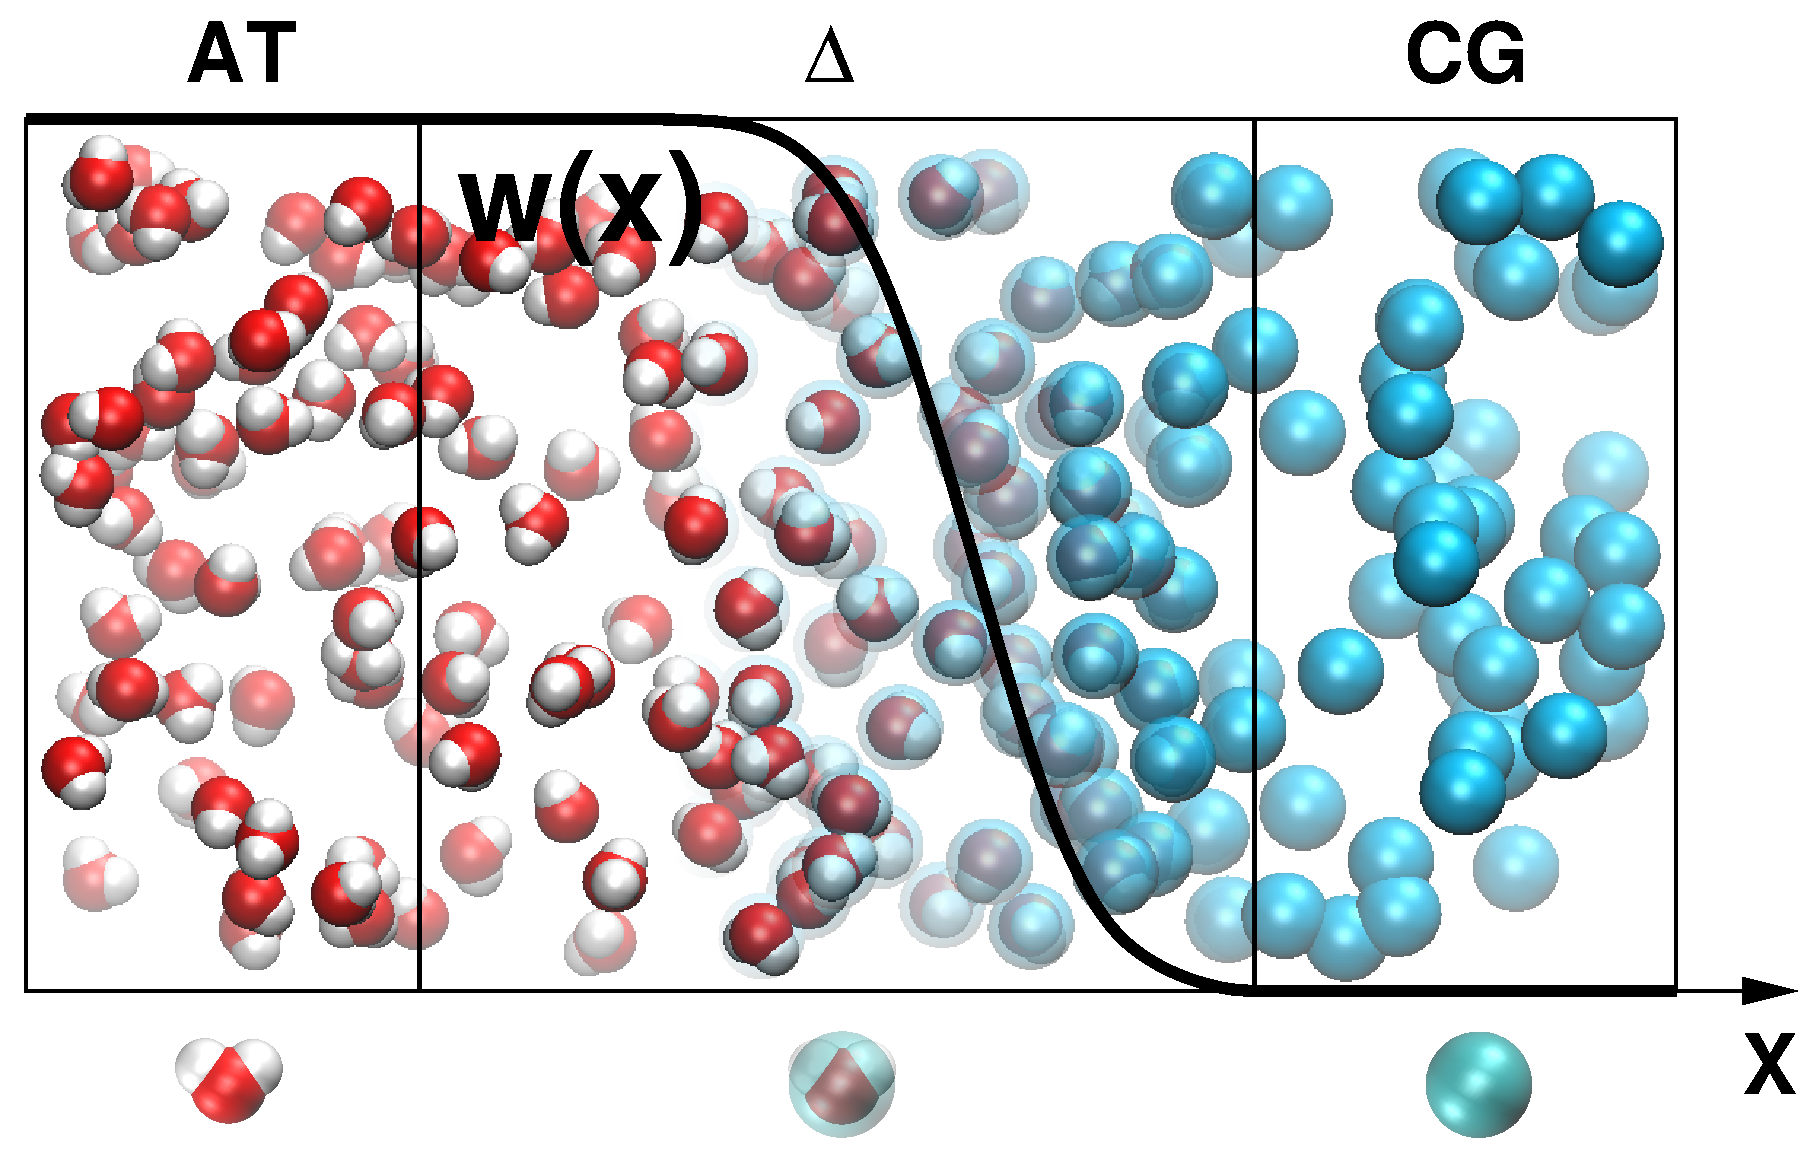
\includegraphics[width=0.8\textwidth]{fig/adapt-wat.eps}
  \end{figure}
  \vfill
\end{frame}

\end{document}
